\documentclass[a4paper,11pt]{article}
\usepackage[margin=1in]{geometry}
\usepackage[czech]{babel}
\usepackage{amsmath}
\usepackage{csquotes}

% package na vklad obrázků
\usepackage{graphicx}
\usepackage{caption}
\usepackage{subcaption}
\usepackage{stfloats} % opravuje obrázky přes celou stránku
\graphicspath{ {./images/} } % definování složky s obrázky

% zvyšování hloubky obsahu
\setcounter{tocdepth}{4}
\setcounter{secnumdepth}{4}

% citace
\usepackage[
    citestyle=numeric,
    autocite=superscript,
    sorting=none
    ]{biblatex} 
% \usepackage{biblatex}
\addbibresource{literature.bib}

\DeclareCiteCommand{\supercite}[\mkbibsuperscript]
  {\iffieldundef{prenote}
     {}
     {\BibliographyWarning{Ignoring prenote argument}}%
   \iffieldundef{postnote}
     {}
     {\BibliographyWarning{Ignoring postnote argument}}%
   \bibopenbracket}%
  {\usebibmacro{citeindex}%
   \usebibmacro{cite}}
  {\supercitedelim}
  {\bibclosebracket}
  
% definování listings pro vklad kódu
% \usepackage{listings}
% \lstset{language=js}

% abstrakt s větším písmem (https://tex.stackexchange.com/a/366170)
\makeatletter
\renewenvironment{abstract}{%
    \if@twocolumn
      \section*{\abstractname}%
    \else %% <- here I've removed \small
      \begin{center}%
        {\bfseries \Large\abstractname\vspace{\z@}}%  %% <- here I've added \Large
      \end{center}%
      \quotation
    \fi}
    {\if@twocolumn\else\endquotation\fi}
\makeatother

\selectlanguage{czech} % nastavení jazyka
% soubor k upřesnění rozdělení slov na slabiky

 % upřesnění slabik v různých cizích slovech

\begin{document}


%%% -------------------- Titulní strana --------------------
\begin{titlepage}
\begin{center}
\large \vspace*{\fill}
\thispagestyle{empty}

\LARGE

{ \huge \textbf{Gymnázium Arabská, Praha 6, Arabská 14}}

{\LARGE Obor programování }

\vfill

\includegraphics{logogyarab.png}
\vspace{15pt}

\vfill

{\huge \textbf{Audiosociální síť: Ding}}

\vfill

Rory Beneš, Kryštof Breburda, Adam Suchý

\vfill

{\large Květen, 2023}

\vspace*{\fill}
\end{center}
\end{titlepage}

%%% -------------------- Prohlášení --------------------
\thispagestyle{empty}
\addtocounter{page}{-1}
\vspace*{\fill}
Prohlašujeme, že jsme jedinými autory tohoto projektu, všechny citace jsou řádně označené a všechna 
použitá literatura a další zdroje jsou v práci uvedené. Tímto dle zákona 121/2000 Sb. (tzv. Autorský zákon) 
ve znění pozdějších předpisů udělujeme bezúplatně škole Gymnázium, Praha 6, Arabská 14 oprávnění k výkonu 
práva na rozmnožování díla (§ 13) a práva na sdělování díla veřejnosti (§ 18) na dobu časově neomezenou a 
bez omezení územního rozsahu.

\vspace{2cm}
V .................. dne .......................

\rightline{Rory Beneš \hspace{0.5cm} ............................ \hspace{2cm}}

\vspace{2cm}

\rightline{Kryštof Breburda \hspace{0.5cm} ............................ \hspace{2cm}}

\vspace{2cm}

\rightline{Adam Suchý \hspace{0.5cm} ............................ \hspace{2cm}}

\vspace{2cm}

%%% -------------------- Anotace --------------------
\newpage
\begin{abstract}
	V rámci tohoto ročníkového projektu jsme vytvořili sociální síť Ding, která je vyhrazena pro zvukové
	nahrávky bez mluveného slova, filtrovaného umělou inteligencí. Ding je webová stránka napsaná v 
	programovacím jazyce JavaScript ve frameworku Vue.js. Serverová část sociální sítě je napsána v jazyce 
	Rust a využívá databázi PostgreSQL.
\end{abstract}

%%% -------------------- Obsah --------------------
\tableofcontents
  % povinné strany

\section{Úvod}
Ding je sociální síť zaměřená na nahrávky zvuků. Mluvené slovo je na síti zakázáno
a automaticky blokováno. Uživatelé se mohou navzájem poslouchat a na své příspěvky
odpovídat.

\subsection{Původní znění zadání}
Cílem by bylo vytvořit sociální síť, na kterou by se nedalo přidat nic jiného
než zvukové soubory, které by nesměly obsahovat mluvené slova (nebo by množství
bylo omezené). Mluvená slova by se automaticky filtrovala. Aplikace by byla
webová stránka.

UI by bylo ve stylu Twitteru, ale upravené pro audio formát. Uživatel by mohl
nahrávat audio hned na webové stránce, nebo nahrát už vytvořený soubor. Měl by
také feed audia od dalších uživatelů.

Později bychom mohli pomocí elektronu udělat android / IOS aplikaci. Primárně
by ale aplikace žila na webu. 

\section{Backend}

Backend, tedy serverová část, je napsána v programovacím jazyce Rust, za využítí knihovny Tide, a
interaguje s PostgreSQL databází. Značna část logiky a integrita je řešena skrz omezení ve schématu
databázových tabulek a skrz ručně napsané SQL příkazy. Frontend se serverem komunikuje pomocí
paradigmatu REST API, přes protokol HTTP, přičemž těla požadavků a odpovědí jsou ve formátu JSON.

\begin{figure}[h!] 
    \centering
    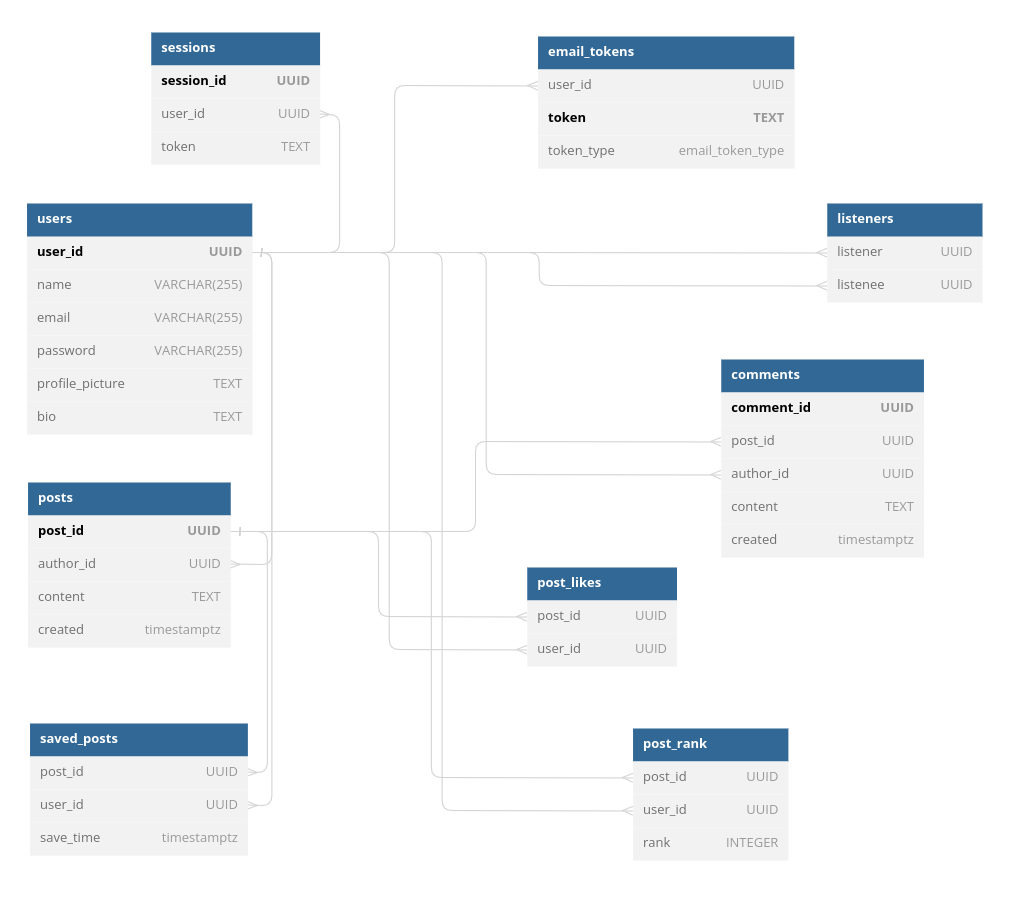
\includegraphics[width=0.8\textwidth]{images/er-diagram.png}
    \caption{ER diagram}
    \label{er-diagram}
\end{figure}

\subsection{Databáze}

Jako databázi jsme zvolili PostgreSQL kvůli rychlosti a množství funkcí, co dokáže. Celkově má
databázové schéma devět tabulek, několik funkcí a náhledů, jak je možno vidět na obrázku
\ref{er-diagram}.

Jedna z výhod PostgreSQL je zabudované full-text vyhledávání, které jsme využili ve funkci
vyhledávání uživatelů. Ve vyhledávání pomocí samotného jména uživatele není full-text vyhledávání
nejlepší metodou, jelikož pracuje s celými slovy, ale velmi se osvědčilo jako sekundární vyhledávání
v celém textu popisku, který si uživatel nastaví.

\subsection{AI rozpoznávání mluvy} \label{backend-ai}

Jeden z hlavních bodů v zadání bylo automatické filtrování mluveného slova. To je možné provést
několika způsoby:

\begin{enumerate}
    \item Analýza frekvencí ve zvukovém souboru.
        \begin{itemize}
            \item Existuje mnoho algoritmu na rozpoznání hlasu, ale ne specificky na mluvené slovo.
            \item Rychlejší, než použití umělé inteligence.
        \end{itemize}
    \item Použití umělé inteligence
        \begin{enumerate}
            \item Využití jednoho z několika veřejných API na rozpoznávání hlasu.
                \begin{itemize}
                    \item Jestliže je nutné API posílat každý příspěvek, pak bude provoz sítě velmi
                        drahý.
                \end{itemize}
            \item Využití již natrénovaného modelu na vlastních strojích. \label{ai-method}
                \begin{itemize}
                    \item Provozovatel sítě musí mít k dispozici stroje, které dokáží příspěvky
                        rychle zpracovat.
                \end{itemize}
            \item Natrénování vlastního rozpoznávacího modelu a jeho užití na vlastních strojích.
                \begin{itemize}
                    \item Provozovatel musí mít hodně prostředků nejen ke zpracovávání příspěvků,
                        ale také ke trénování modelu.
                \end{itemize}
        \end{enumerate}
\end{enumerate}

Pro Ding jsme zvolili variantu \ref{ai-method}. Pro rozpoznávání mluveného slova používáme AI model
"Whisper AI" od americké společnosti OpenAI \cite{openai-whisper}. Tento model je veřejně přístupný
a je možné si ho spustit na osobním počítači, nebo serveru. Původní model velmi využívá GPU na
grafické kartě počítače. Většina serveru ale grafické karty nemá a tudíž je nutné výpočty provádět
na samotném CPU. Tento problém řeší projekt whisper.cpp od Georgiho Gerganova, který model upravil
tak, aby ho bylo možné spustit na mnohem slabších zařízeních, než jsou speciální počítače OpenAI.

Při přidání nového příspěvku se tedy nejdříve zvukový soubor zkontroluje, že je funkční a ve
správném formátu. Dál se využije AI modelu pro přepsání jakéhokoliv mluveného slova. Pokud je
příspěvek v nesprávném formátu, nebo v něm model najde slova, pak je zpětně smazán. Je tedy možné,
že na pár vteřin (nebo minut, záleží na zatížení stroje), bude příspěvek přístupný, i když by měl
být smazán.

\subsection{E-mail a odložené úkoly}

Ding je navržen tak, aby každý požadavek čekal co nejkratší dobu. Například na vyslání e-mailu, nebo
kontrolu příspěvku (popisována v sekci \ref{backend-ai}) požadavek nemusí čekat. Knihovna Tide tuto
vlastnost nemá zabudovanou a bylo tedy potřeba si vytvořit vlastní systém pro odbavování těchto
"odložitelných" úkolů.

Celá aplikace běží v asynchronní smyčce, což umožňuje aplikaci dělání více věcí najednou. Narozdíl
od čistého programování s vlákny není paralelizace "pravá". V asynchronní smyčce může být mnoho
úkolů, které se mají konat, a procesor mezi nimi přepíná (obrázek \ref{async-diagram}). V tradičním
programování s vlákny beží všechny úkoly najednou na více procesorových jádrech, nebo se o přepínání
stará operační systém. Operační systém však neví, kdy se aplikaci hodí, či nehodí, aby procesor
přepnul mezi úkoly, a programátor si musí hlídat, aby dvě vlákna neupravovala informace na jednom
místě. V asynchronním programování je tento problém značně zredukovaný, jelikož procesor mezi úkoly
přepíná jen při klíčovém slově \texttt{await}.

\begin{figure}[h!] 
    \centering
    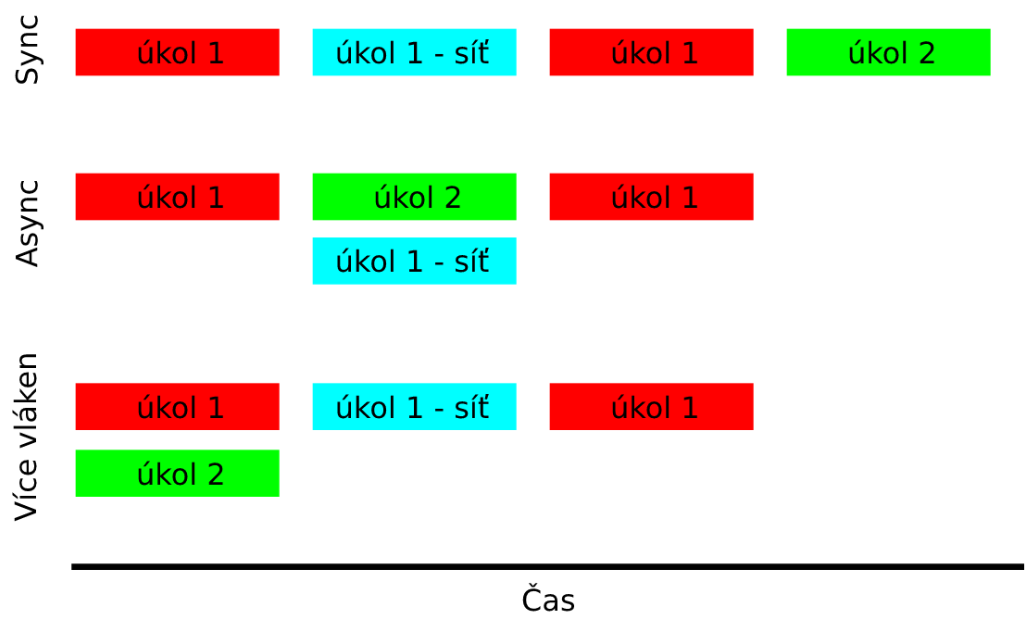
\includegraphics[width=0.6\textwidth]{images/async.png}
    \caption{Synchronní, asynchronní a vícevláknové programování}
    \label{async-diagram}
\end{figure}

\subsection{Autentizace uživatelů}

Autentizace uživatelů je provedena přes relační tokeny. Aby uživatel dostal token pro svou relaci,
musí vyslat požadavek \texttt{POST /api/sessions} se svými přihlašovacími údaji (email, heslo).
Backend tyto údaje ověří vůči informacím v databázi a jestliže souhlasí, pak vytvoří pro uživatele
nový relační token, který složí k autentizaci a identifikaci dalších požadavků. Tento token si
prohlížeč ukládá v paměti \texttt{window.localStorage}.

Před uložením do databáze jsou hesla zahašována algoritmem \texttt{PBKDF2} se \num{100 000} iteracemi. V
databázovém sloupci s heslem je také uložena sůl použita při hašování a informace o hašovacím
algoritmu pro případ, že by bylo algoritmus potřeba v budoucnu změnit.


\newpage
\printbibliography
\listoffigures

\end{document}
